\documentclass[a4paper]{article}

\usepackage[spanish]{babel}
	\selectlanguage{spanish}
\usepackage{geometry}
	\newgeometry{margin=3cm}
\usepackage{setspace}
\usepackage{graphicx}
\usepackage{float}
\usepackage[utf8]{inputenc}

\title{Reporte del Producto 7}
\author{Ana Gabriela Carretas Talamante}
\date{11 de mayo de 2015}

\begin{document}
\maketitle
\section{Introducción}
En este último reporte, se presentará el análisis de un conjunto de series de tiempo referidos a propiedades de ciertas mareas, proporcionado el Dr. Julio César Rodríguez, del Departamento de Agricultura. Los datos corresponden al manglar El Sargento, ubicado en la costa, cerca del Desemboque de los Seris, casi frente a la Isla del Tiburón. El objetivo es, presentar gráficamente el comportamiento de las mareas y estimar el intervalo de tiempo promedio para cada tipo de marea.
 
\section{¿Qué son las mareas?}
Conocemos por Marea al movimiento periódico y alternativo de ascenso y descenso del nivel del mar, producido por las acciones atractivas del Sol, la Luna y demás cuerpos astrales, que se repite cada 12 horas 24 minutos. Su intensidad está en íntima relación con las posiciones relativas que el Sol y la Luna tienen respecto a la Tierra. Es imposible hacer de este complejo fenómeno una descripción general y completa, pues de un lugar a otro en el globo terrestre, varían de tal modo sus características, que es difícil por ellas solamente afirmar que siempre tiene el mismo origen.

\subsection{Un poco de historia}
El fenómeno de mareas es conocido desde la antigüedad. Parece ser que Piteas fue el primero en señalar la relación entre la amplitud de la marea y las fases de la Luna, así como su periodicidad. Plinio el Viejo en su \textit{Naturalis Historia} describe correctamente el fenómeno y piensa que la marea está relacionada con la Luna y el Sol. Mucho más tarde, Bacon, Kepler y otros trataron de explicar ese fenómeno, admitiendo la atracción de la Luna y del Sol. Pero fue Isaac Newton en su obra \textit{Principios de la Filosofía Natural} quien dio la explicación de las mareas aceptada actualmente. Más tarde, Pierre-Simon Laplace  y otros científicos ampliaron el estudio de las mareas desde un punto de vista dinámico.

\begin{figure}[H]
    \centering
    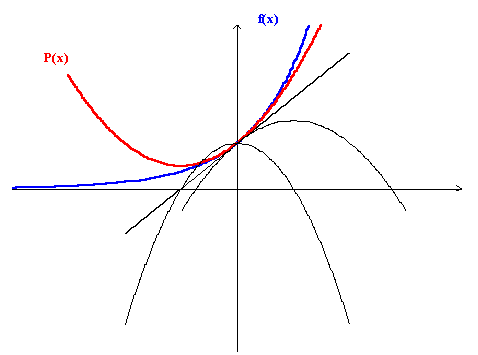
\includegraphics[width=11cm]{1}
  \end{figure} 
\newpage
\subsection{Clasificación de las mareas}
A continuación se recogen los principales términos empleados en la descripción de las mareas:
\subparagraph{Por su altura} 
  \begin{itemize}
  \item \textbf{Marea alta o pleamar:} Momento en que el agua del mar alcanza su máxima altura dentro del ciclo de las mareas.
  \item \textbf{Marea baja o bajamar:} Momento opuesto, en que el mar alcanza su menor altura.
  \end{itemize}
  El tiempo aproximado entre una pleamar y la bajamar es de 6 horas 12 minutos, completando un ciclo de 24 horas 50 minutos.
  
\subparagraph{Según su movimiento horizontal o corrientes de marea}
  \begin{itemize} 
  \item \textbf{Flujo o marea entrante:} Se trata de un lento y continuo ascenso hacia aguas marinas, generalmente influido por la luna y el sol, cuando se encuentra luna nueva o luna llena.
  \item \textbf{Reflujo o marea saliente:} Debido a que la atracción lunar es poca o nula, la corriente marina se ve en estado saliente de manera lenta y progresiva.
  \end{itemize}
  
\begin{figure}[H]
    \centering
    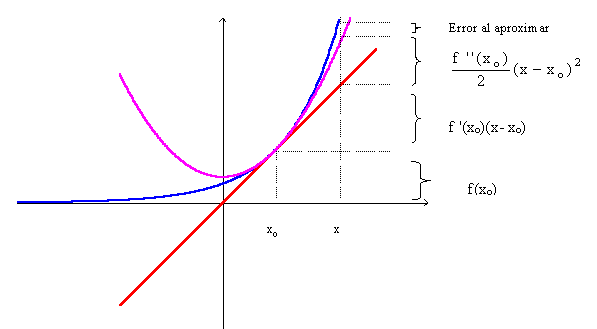
\includegraphics[width=11cm]{2}
  \end{figure} 

\subparagraph{Según la geografía del lugar y el tipo de viento que predomina}
  \begin{itemize}
  \item \textbf{Semidiurnas:} Durante el transcurso de un día lunar pueden observarse dos pleamares y dos bajamares. El día lunar cuenta con 24 horas y 50 minutos, es decir que cada 6 horas y 13 minutos se produce un aumento en la marea o una baja en la marea. 
  \item \textbf{Diurnas:} Esta marea es típica de una zona con una latitud baja. Cuenta con una pleamar y una bajamar en un día lunar, por lo que se aprecia una subida del nivel del mar o una bajada del nivel del mar cada 12 horas y 25 minutos.
  \item \textbf{Diurnas irregulares:} Cuenta con dos ciclos a nivel de cambios en las mareas, es decir, con una pleamar y una bajamar, pero estos cambios se producen con diferentes alturas y diferentes periodos de tiempo.
  \item \textbf{Mareas mixtas:} Estas mareas no cuentan con un sólo rango específico, ya que en un día lunar pueden encontrarse tanto dos bajamar y dos pleamar, como una sola subida del nivel del mar y una sola bajada del nivel del mar.
  \end{itemize}

\subsection{Teoría de mareas}
La teoría de las mareas es la aplicación de la mecánica para interpretar y predecir las deformaciones de marea de cuerpos planetarios y satélites y sus atmósferas y océanos bajo la carga gravitatoria de otro cuerpo astronómico. \\

En 1616 Galileo escribió \textit{"Diálogo"} basándose en la teoría que finalmente demostraría ser falso). En el se pretendía encontrar la prueba física del doble movimiento diario y anual de la Tierra exigido por el sistema copernicano. \\

La solución propuesta por Galileo se basa en la analogía entre el fenómeno comúnmente observado de las oscilaciones del agua contenida en un recipiente sometido a fases de aceleración y desaceleración y las oscilaciones de los mares sobre la superficie del globo terrestre. \\

Newton fue el que proporcionó una explicación correcta de la fuerza de las mareas. Esta puede utilizarse para explicar las mareas en un planeta cubierto por un océano uniforme, pero sin tomar en cuenta la distribución de los continentes o batimetría oceánica.

\section{Analizando los datos}
Los resultados presentados para los diferentes ciclos en la región estudiada, fueron los siguientes:
\begin{table}[h!]
  \centering
  \begin{tabular}{|p{3cm}|p{3cm}|}
  \hline
 Ciclo lunar&29.2500000 días\\ \hline
 Marea diurna&1.00158226 días \\ \hline
 Marea semidiurna&0.500000000 días \\ \hline
   \end{tabular}
  \end{table} 

que con sus debidas transformaciones en horas y minutos, tendremos los resultados de la siguiente manera:
\begin{table}[h!]
  \centering
  \begin{tabular}{|p{3cm}|p{3cm}|}
  \hline
 Ciclo lunar&29 días 6 horas \\ \hline
 Marea diurna&24 horas \\ \hline
 Marea semidiurna&12 horas 1 minuto \\ \hline
   \end{tabular}
  \end{table} 

\begin{figure}[H]
    \centering
    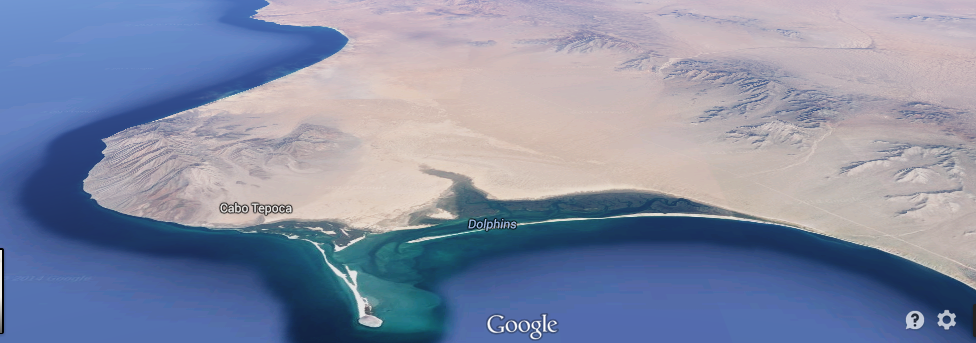
\includegraphics[width=14cm]{3}
  \end{figure} 
  
Se presentarán a continuación las gráficas obtenidas después del refinamiento de datos con el código anexo en la carpeta del repositorio.

\subsubsection{Gráfica \#1}
\begin{figure}[H]
    \centering
    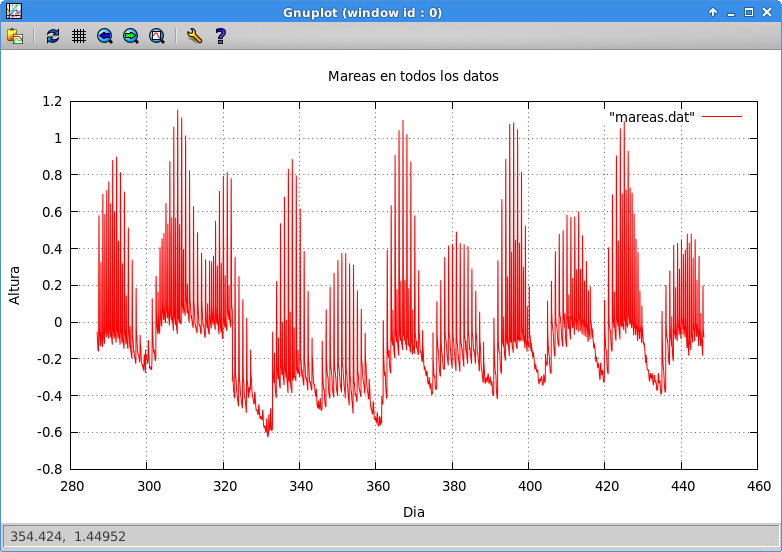
\includegraphics[width=12cm]{11} \\
  \end{figure} 
En esta gráfica se muestran los altibajos por las mareas de todos los días brindados por el archivo de datos. En los días, se tiene que a partir del día 1, por efectos de continuidad con el conteo, se le sumaron los 365 día anteriores. Se puede notar la forma en que varía la marea según la fase en la que está.

\subsubsection{Gráfica \#2}
\begin{figure}[H]
    \centering
    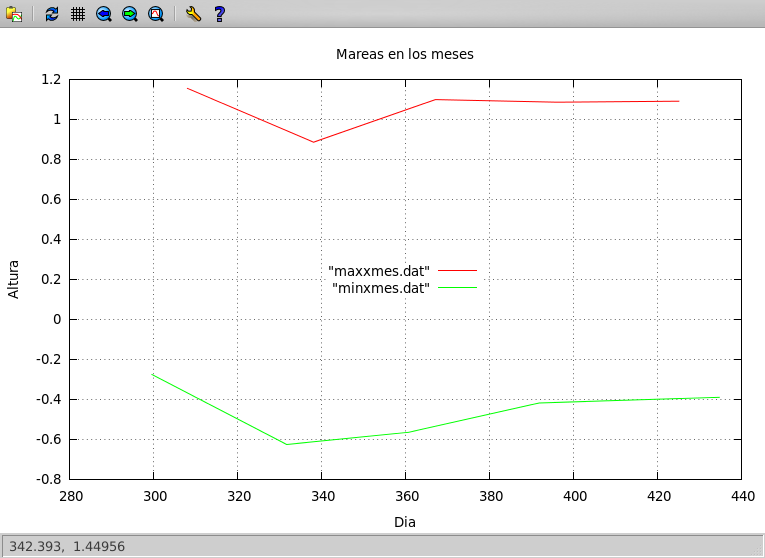
\includegraphics[width=12cm]{22} \\
  \end{figure} 
Son 5 picos los que muestra la gráfica, comparando los máximos y mínimos de los meses de utilidad total. Se puede notar que están ligeramente intercalados, debido a la misma clasificación de mareas.

\subsubsection{Gráfica \#3}
\begin{figure}[H]
    \centering
    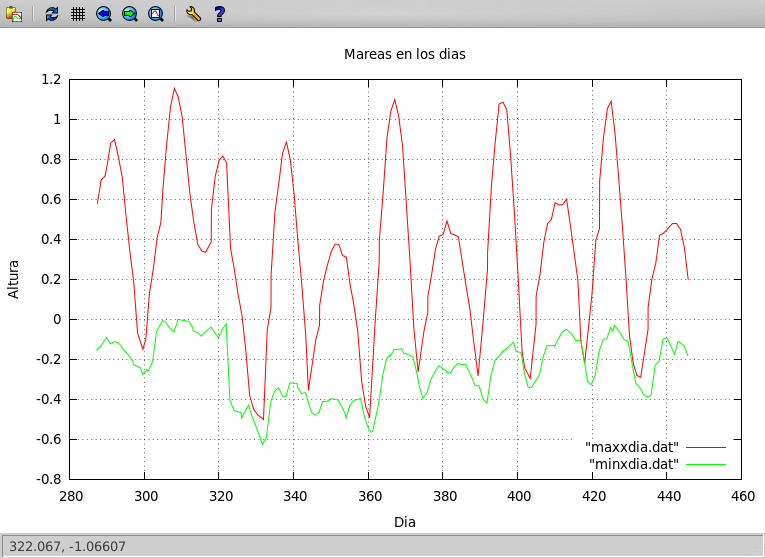
\includegraphics[width=12cm]{33} \\
  \end{figure} .
Se pueden notar las mareas altas altas y las bajas bajas, diferenciadas por la misma gráfica. Esta es la comparación de máximos y mínimos en todos los días de datos.

\section{Conclusión}
En esta práctica podemos concluir que la física tiene diversas aplicaciones en donde podemos utilizar recursos distintos para poder obtener cierto resultado. En este caso, recurrimos a la tecnología de la programación para aligerarnos el trabajo. Claramente podríamos buscar manualmente alguna coincidencia, pero eso llevaría muchísimo tiempo y no generaría resultados totalmente buenos. Así que, la programación es una herramienta básica en el campo de observación y cuantificación de datos, como lo realizado en esta práctica. \\

Las mareas son un fenómeno muy interesante por su periodicidad, brindan bastante utilidad y además sirven como comprobación de diversas teorías de gravitación.
\end{document}
